\documentclass{article}

\usepackage{paper}

% Can work with lesser data for pre-training (TEST THIS OUT)

\setpapertitle{Incremental Training of a Two Layer Neural Network}
\setauthor[guggu@iitk.ac.in]{Gurpreet Singh}{150259}
\addauthor[jkapoor@iitk.ac.in]{Jaivardhan Kapoor}{150300}

\renewcommand{\makeheader}{
	\begin{center}
		\parbox{0.9\textwidth}{%
			\hrule height4pt
			\vspace{5mm}

			\begin{center}
				\setstretch{1.5}
				{\fontsize{16pt}{20pt} \bt{\papertitle}}
			\end{center}

			\vspace{3mm}
			\hrule height2pt
		}

		\vspace{5mm}

		\begin{center}
			\bt{\fontsize{11}{11}\selectfont \ut{Group 10}}
		\end{center}


		\parbox{0.75\textwidth}{
			\begin{center}
				\authors
			\end{center}
		}
	\end{center}
}

\begin{document}
\makeheader

\abstract{
	Gradient boosting for convex objectives has had a rich history and literature with provable guarantees for many years now. The same cannot be said for the workings of a neural network, while the class of neural networks is a set of incredibly powerful models, which can approximate complex function mappings. In this project, we make an attempt to combine the two approaches with a boosted model as a warm start for a single layer neural network, with provable convergence guarantees. We also see how gradient boosting on single node single hidden layer network essentially corresponds to sequential training of hidden layer nodes, and therefore can be used as a starting point for application of the backpropagation scheme for better results. Among these, we also look at the convergence analysis of functional gradient descent, which is used to train the weak learners, or nodes in our case, and empirical results received thereafter.
}

\begin{psection}{Introduction}

	Feed Forward Neural Networks are incredible function approximators. However, there are a few caveats when it comes to training a neural network. Firstly, there is less on the proper initialization of the neural network nodes to ensure convergence. Also, the most common method of optimization is Stochastic Gradient Descent, which although provably converges to the global optima in finite steps (for finite optimal points), offers no such guarantees in case of non-convex functions, and since a neural network is a multi-level mapping of non-linear functions, the objective is highly non-convex. Therefore, SGD methods only work as heuristics in the case of neural networks.

	We attempt to remedy this, up to a certain sense, by incrementally training a neural network. Although we look at only single hidden layer neural networks, it is possible to extend the theory to multiple layers as well, but the complexity of training would increase in that case.

	The essential motivation behind this is that a single hidden layer neural network can be thought of as an ensemble of multiple nodes, which in our analogy become the weak learners, and the whole network as an ensemble or mixture of these weak learners. This analogy allows us to compare neural networks with other ensemble techniques, such as bagging and boosting. Since the weak learners in our case are essentially single node in a single hidden layer network, the learners have very high bias, and since bagging relies on the bias of each learner, we cannot find much use of it.

	However, the method of boosting fits very naturally in our problem setting, where we can learn one node (one weak learner) on the input data, and learn the next node on the residual of this node, and the next on the residual of the second node, and so on. This allows us to incrementally train each node, where one node communicates with a previous node only through the residuals. Throughout the text, we refer to the boosting method as incremental training of the neural network, and the standard backpropogation scheme as the collective training of the neural network.

	We first give a brief background of the tasks we have at hand, and then a brief history of boosting and a sketch of how we use boosting for our training. Later, we move on to an empirical comparison between incremental training and collective training of a neural network.

\end{psection}

\begin{psection}{Relevant Background}

	\begin{psubsection}{Function Estimation}

		In the function estimation problem, we usually have a set of tuples of data points, and labels or response variables, commonly denoted by $\vx \in \cX$ and $y \in \cY$ respectively. We assume these tuples to be generated from a data distribution $\cD$, which is unknown to us, and the goal is to estimate a function $f : \cX \ra \hat{\cY}$ such that the error or risk (defined below) is minimized.

		\begin{definition}[Risk]
			\label{def:risk}
			The risk for a function estimate is given with respect to a loss function $l : \cY \times \hat{\cY} \ra \bR$ and a data distribution $\cD$, and is defined as
			\begin{align*}
				\rgrt[_\cD^l]{f} \qdeq \E[\vX, \sY \sim \cD]{\func{l}{\sY, f(\vX)}}
			\end{align*}
		\end{definition}

		The choice of loss function depends on the problem we wish to solve, and the range of the response variable $\cY$ and the function range $\hat{\cY}$. For example, if the response variable and the function range, both are Bernoulli variables, then an apt choice of the loss function is $0-1$ loss, which is given as $l^{0-1}(Y, \wY) \deq \is{Y = \wY}$.

		We can now formally define the goal of a function estimation problem. Given a data distribution $\cD$, where random variables $\vX \in \cX$ and $\sY \in \cY$ are draw from this distribution, we wish to estimate a function $f^\ast : \cX \ra \hat{\cY}$ such that the following holds
		\begin{align*}
			f^\ast \qdeq \argmin{f} \E[\vX, \sY \sim \cD]{l(\sY, f(\vX))}
		\end{align*}

		\begin{pssubsection}{Working with Finite Data}

			Since we do not actually know the data distribution, it is impossible to find a function to minimize with respect to the data distribution. We therefore find a surrogate objective to minimize, and ensuring, under certain conditions \footnote{\ Some sufficient conditions are stability of the Loss function or Uniform Convergence of the hypothesis space. Details can be found in \cite{uml-tta}}, that the proxy function we found using the surrogate objective is representative of the function $f^\ast$, where $f^\ast$ is as defined earlier.

			The surrogate objective is defined as follows
			\begin{align*}
				\hat{f} \qdeq \argmin{f} \frac{1}{\abs{\cS}} \sum_{\vx, y \sim \cS} l(y, f(\vx))
			\end{align*}
			where the set $\cS \deq \set{(\vx^n, y^n)}_{n = 1}^N$ is sampled from the data distribution $\cD^N$ identically and independently.

			The objective to minimize in the above expression is known as the empirical risk with respect to a sample set, and is formally given as
			\begin{align*}
				\rgrt[_\cS^l]{f} \qdeq \frac{1}{\abs{\cS}} \sum_{\vx, y \sim \cS} l(y, f(\vx))
			\end{align*}

			\begin{remark}
				The term on the RHS of the above optimization objective is defined as the empirical risk, denoted by $\cR_\cS^l$.
			\end{remark}

			\begin{note}
				For the remaining text, we assume that we have a sample set $\cS$ sampled i.i.d. from the data distribution which is used for the purposes of training. This is also known as the training set.
			\end{note}

		\end{pssubsection}

		\begin{pssubsection}{Working with Restricted Hypothesis Classes}

			Since the objectives described above are over unconstrained spaces, we can achieve minimum error by minimizing the error point-wise, however this is usually not desired. Therefore, we limit the minimization over a restricted Hypothesis Space, denoted by $\cF$. This allows us to control the function class over which we optimize, and better analyze the algorithm. Hence, our new objective becomes
			\begin{align*}
				\hat{f} \eq \argmin{f \in \cF} \frac{1}{N} \sum_{(\vx, y) \in \cS \sim \cD^N} \func{l}{y, f(\vx)}
			\end{align*}

		\end{pssubsection}

	\end{psubsection}

	\begin{psubsection}{Gradient Descent}

		Gradient Descent \citep{gd-original} or \et{Steepest Descent} is a method to optimize (minimize) convex objectives, usually where a closed form solution is either not available or slow to compute analytically. For example, consider the objective of logistic regression, where no closed form solution is available. Therefore, we need numerical methods to reach the optimal value, $\hat{f}$.

		Assume we have a convex objective $\vPhi$ to be minimized over a variable $\vx \in \cX$. A vanilla gradient descent step for the given setting looks like the following
		\begin{enumerate}
			\item First, the gradient $\vg_t$ at the current time step $t$ is computed as
				\begin{align*}
					\vg_t &\qdeq	\brac{\nabla_\vx\,\vPhi(\vx)}_{\vx = \vx_t} \\[.2em]
					&\eq			\brac{\derp{\vPhi(\vx)}{\vx}}_{\vx = \vx_t}
				\end{align*}
			\item The current estimation of the optimal point $\vx_t$ is updated using the negative gradient weighted with a step value $\eta_t$ as follows
				\begin{align*}
					\vx_{t + 1} \eq \vx_t - \eta_t \cdot \vg_t
				\end{align*}
		\end{enumerate}

		Gradient Descent offers good convergence guarantees for convex objectives, and better for strongly-convex and/or strongly-smooth objectives. We have discussed this is detail in our survey of \et{Gradient Descent and its Variants}.

	\end{psubsection}

	We now move on to Boosting Methods, especially Gradient Boosting in the next section.

\end{psection}

\begin{psection}{Generic Boosting Algorithms for Convex Optimization}

	\begin{definition}[Boosting]
		Boosting is a machine learning ensemble meta-algorithm for primarily reducing bias and variance \citep{boost-var} in supervised learning, and a family of machine learning algorithms which combine multiple weak learners to form a superior strong learner\footnote{\ Source: \url{https://en.wikipedia.org/wiki/Boosting_(machine_learning)}}.
	\end{definition}

	AdaBoost \citep{adaboost} was the first successful boosting algorithm designed for classification tasks. AdaBoost uses decision stumps as weak learners and each weak learner is trained on the same data samples with the loss weighted by the rate of mis-classification for each data point. \cite{adaboost} showed that AdaBoost in fact converges and provided an upper bound on the risk for the combined classifier. In fact, only algorithms that provably converge in the PAC framework can be classified as boosting algorithms.

	Many other boosting algorithms exist for problem specific tasks exist, such as LPBoost, TotalBoost, BrownBoost, LogitBoost, etc. exist. \cite{gbm} provided a generic technique for boosting algorithms which provides general methods for application in any supervised learning setting with a convex objective.

	\et{Friedman} in his paper proposed a novel boosting algorithm, known as Gradient Boost which is very closely related to the method of Gradient Descent, and therefore enjoys the convergence properties of Gradient Descent, although not directly.

	Although there are other general boosting algorithms such as AnyBoost and DOOM proposed by \cite{anyboost}, we exclude them from our report, since Gradient Boost fits more naturally into our paradigm. We discuss the Gradient Boost Algorithm in detail in the following sections.

	\begin{psubsection}{Gradient Boost}

		For the standard Boosting Methods, we restrict the form of the function $\hat{f}$ to be an additive function, \ie we restrict $\hat{f}$ such that there exist functions $\set{f_m \in \cH}_{m = 1}^M$ where $\cH$ is a subset of the hypothesis space of $\hat{f}$ ($\cH \in \cF$) and values $\set{\beta_m \in \bR}_{m = 1}^M$, we have
		\begin{equation}
			\hat{f} \eq \sum_{m = 1}^M \beta_m f(\vx; \va_m)
		\end{equation}
		where for each $m \in \brac{M}$, $\va_m$ represent the set of parameters that define the m\tth component of the function $\hat{f}$.

		\begin{remark}
			It is not necessary for the $\hat{f}$ to be in the hypothesis space $\cH$ since the space might not be closed under addition or scalar multiplication, or both.
		\end{remark}

		This is termed as an additive model, and boosting essentially builds an additive model. \cite{additive} showed that even AdaBoost builds an additive model, even though there is no explicit notion of additive modeling within AdaBoost.

		Since we want to minimize the empirical risk defined in Section 2.1.1, we can write the objective $\vPhi : \cF \ra \bR$ as
		\begin{align*}
			\vPhi(f) \qdeq \frac{1}{N} \sum_{(\vx, y) \in \cS \sim \cD^N} l(y, f(\vx))
		\end{align*}
		and the optimal point is given as $\hat{f} = \argmin{f \in \cF} \vPhi(f)$.

		Since we know that the opimal point is an additive model, we can replace the objective as
		\begin{align*}
			\set{\beta_m, \va_m}_{m = 1}^M \eq \argmin{\set{\beta_m, \va_m}_{m = 1}^M} \func{\vPhi}{\sum_{m = 1}^M \beta_m f(.\,;\va_m)}
		\end{align*}

		However, for most objectives, this does not give a closed form solution. Therefore, we need to apply alternate methods to optimize $\vPhi$. A proposed method is to compute the individual components greedily, \ie we keep adding a component $\beta_m f(.\,; \va_m)$ to $\hat{f}$ until convergence.

		This is greedy stage wise procedure, where the current estimate, \ie at time step $m - 1$, of $\hat{f}$ is given by $\hat{f}_{m - 1}$, and the update step for the stage wise procedure can be written as two steps, given below
		\begin{align*}
			\beta_m, \va_m	&\eq	\argmin{\beta, \va} \vPhi(\hat{f}_{m - 1} + \beta f(.\,; \va)) \\
			\hat{f}_m		&\eq	\hat{f}_{m - 1} + \beta_m f(.\,; \va_m)
		\end{align*}

		At this point, a resemblance can be seen between the above updates and the method of Gradient Descent \citep{fgt, gbm}. In fact, Gradient Boosting is essentially a combination of Gradient Descent and Boosting. Comparing the above update step to the update step of gradient descent, one can be convinced that replacing the $m$\tth component of $\hat{f}$ or the update of the function $\hat{f}_{m - 1}$ can be replaced by the gradient of the objective with respect to the update component, and replace $\beta_m$ with the step value at time step $m$.

		More formally, we replace the update steps as follows
		\begin{enumerate}
			\item Compute the gradient of the minimizing objective $\vPhi$ as
				\begin{align*}
					g_{m - 1} \eq \brac{\derp{\vPhi(f)}{f}}_{f = \hat{f}_{m - 1}}
				\end{align*}
			\item The function estimate is then updated as
				\begin{align*}
					\hat{f}_m \eq \hat{f}_{m - 1} - \eta_m g_{m - 1}
				\end{align*}
		\end{enumerate}

		From the ideas of gradient descent, we can expect this to converge to the global optima in case the objective is convex with respect to the function space $\cF$ or even the space covered by functions represented as an additive model.

		We still have one problem to solve. The gradient in this case is a function. And in order to minimize the empirical risk, we minimize the loss function point-wise. Therefore, at a data point $(\vx, y)$, we want the value of the gradient $g_m(\vx, y)$ to be such that we take a maximum descent step from the current function estimate, at this point. More formally, we want the value of the gradient at point $(\vx, y)$ to be such that
		\begin{align*}
			g_m(\vx, y) \eq \brac{\derp{l(y, f(\vx))}{f}}_{f = \hat{f}_{m}}
		\end{align*}
		as this would allow us to take steepest descent step for each data point.

		Now, since the values of the gradient at any time step depend on the data points in the set $\cS$, we only know the actual value of the gradient at these points. Therefore, instead of having a complete function, we have the value of the gradient function at a finite set of points $\cS$.

		This motivates us to approximate this gradient using another function, which is to be learned. This is the point where the notion of weak learners come in. We approximate or estimate the gradient using a function $h_m \in \cH$ which belongs to a restricted hypothesis class. This function $h_m$ acts as a proxy for the gradient $g_m$ and therefore is used to update the function estimate $\hat{f}_{m - 1}$ at the previous time step. We define the function $h_m$ to be as follows
		\begin{equation}
			h_m \qdeq \argmax{h \in \cH} \frac{\dotp{g_m}{h_m}}{\norm{h_m}}
			\label{eq:weak-obj}
		\end{equation}
		where the dot product and norm is defined over the $\sL^2$ function space (defined later). If the hypothesis space $\cH$ is closed under scalar multiplication, the objective becomes \citep{cvx-boosting}
		\begin{equation}
			h_m \qdeq \argmax{h \in \cH} \norm{h_m - g_m}^2
			\label{eq:weak-obj-closed}
		\end{equation}

		Since we do not have the data distribution, we cannot actually compute the dot product or the norm in the $\sL_2$ space, we approximate the objective using the sample set $\cS$, which allows us to know the values of $g_m$ at those points as well as find a good proxy function from the restricted hypothesis space.

		This method is known as \et{Restricted Gradient Descent} where we use a surrogate to the gradient to make the actual gradient step.

		The step is chosen either using Heuristics, or using line search, where the optimal value of $\beta_m$ is computed such that the update minimizes the loss. The complete algorithm for Gradient Boost is given in Algorithm \hyperlink{algo:1}{1}. We formalize the notion of Restricted Gradient Descent and Gradient Boosting in the next section, while giving a convergence bound for the same.

	\end{psubsection}

	\begin{algo}[0.8\textwidth]{Gradient Boost}

		\bt{Input:} \quad a sequence of data points $\cS \sim \cD^N$ and a loss function $l : \cY \times \hat{\cY} \ra \bR$ \sbr

		\bt{Output:}\, $\hat{f}$, an estimate of the optimal function

		\bt{Steps:}

		\begin{enumerate}
			\item Initialize $\hat{f}_0 \in \cH$
			\item For $m = 0 \dots M - 1$ or until convergence, do
				\begin{align}
					\qforall n \in \brac{N}, \quad g_{m, n}	&\eq	\brac{\derp{l(y_n, f(\vx_n))}{f}}_{f = \hat{f}_{m}} \tag{Gradient Step} \\
					h_m										&\eq	\argmax{h \in \cH} \frac{\dotp{g_m}{h_m}}{\norm{h_m}} \tag{Weak Learning Step} \\
					\hat{f}_{m + 1}							&\eq	\hat{f}_m - \beta_m h_m \tag{Update Step}
				\end{align}
				where $\beta_m$ is equal to $\eta_m \cdot \frac{\dotp{g_m}{h_m}}{\norm{h_m}}$ and $\eta_m$ is obtained using line-search or using a heuristic step value.
			\item Return $\hat{f} = \hat{f}_M$
		\end{enumerate}
		Initialize a function $\hat{f}_0$

	\end{algo}

	\begin{psubsection}{Convergence Analysis of Gradient Boost}

		We refer to \cite{cvx-boosting} for the convergence analysis of the Restricted Gradient descent method used for the objective here. The cited work contains some relevant definitions which we shall restate here for completeness. We shall then proceed to state theorems on convergence guarantees in regards to the notation thus introduced.

		\begin{pssubsection}{$L^2$ Function Space}

			\cite{functionspace} proposed that the $L^2$ function space is a natural match for analyzing the convergence of gradient descent. For an input domain $\cX$, an output vector space $\cV$, and a measure $\mu$, the $L^2(\cX, \cV, \mu)$ space is defined as the set of functions $f : \cX \ra \cV$ such that the following Lebesgue integral is finite.
			\begin{align*}
				\int_{\cX} \norm{f(\vx)}^{2} \id \mu \qlt \infty
			\end{align*}

			If $\mu$ is a probability measure, then the above can be written as an expectation $\E[P]{\norm{f(\vx)}}$. The $L^2$ space is a Hilbert space, with the inner product given as
			\begin{align*}
				\dotp{f}{g}_P &\eq	\int_{\cX} \dot{f(\vx)}{g(\vx)}_{\cV} P(\vx) \id \vx \\
				&\eq				\E[P]{\dotp{f(\vx)}{g(\vx)}_{\cV}}
			\end{align*}
			and
			\begin{align*}
				\norm{f}_P^2 &\eq \dotp{f}{f}_P
			\end{align*}

			If only a set of samples (say $\cS_P$) are available from the measure $P$, we can replace the expectation using these samples as
			\begin{align*}
				\dotp{f}{g}_P^2 \eq \frac{1}{N} \sum_{\vx \in \cS_P} \dotp{f(\vx)}{g(\vx)}_{\cV}
			\end{align*}

		\end{pssubsection}

		\begin{pssubsection}{Aligning Power of a Hypothesis Space}
			We will consider the Hilbert space of functions in the empirical space $\hat{P}$, where the inner product is defined as
			\begin{align*}
				\langle f,g\rangle=\frac{1}{N}\sum_{n=1}^N\langle f(\vx_n),g(\vx_n)\rangle
			\end{align*}
			From the above algorithm, we see that the ideal direction for the gradient to move in the restricted space, is the learned weak learner. We can interpret as performing GD in the function space, to minimize the value of the functional (in this case the loss function). Since the empirical space is restricted, there are only a restricted number of directions we can move. The best direction is given by the weak learner that is learned at every step.

			We define the "aligning power" of the hypothesis space $\cH$ (the restricted space of the weak learners), the ability of it to align to the real gradient of the functional. This is also known as the edge of the hypothesis space. We present the formal definition of edge as given by \cite{cvx-boosting}.
			\begin{definition}[Edge]
				A restricted set $\cH$ has edge $\gamma$ if $\qforall \vg$, $\exists h \in \cH$ such that $\dotp{g}{h} \ge \gamma \norm{g} \norm{h}$
			\end{definition}
		\end{pssubsection}

		\begin{pssubsection}{Convergence Bound}

			We assume that the hypothesis space for the weak learners is a proper subset of the $L^2(\cX, \cY, \cD)$ where $\cX$ is the vector space of the input featues, $\cY$ is the vector space of the output vectors and $\cD$ (a probability measure) defines the underlying data distribution we assume. Below we analyze the convergence in case the risk functional is strongly convex and strongly smooth for the Gradient Boosting Algorithm given in \hyperlink{algo:1}{Algorithm 1}.

			Also, since we do not have the data distribution, we find the convergence of the empirical risk with respect to the sample set $\cS$. To ensure convergence, between the empirical risk and the real risk, statistical analysis must be down, but we do not cover that in this report.

			\begin{theorem}
				Let $\rgrt[_\cS^l]{.}$ be a $\lambda$-strongly-convex and $\beta$-strongly-smooth functional over the $L^2$ space given by the tuple $(\cX, \cY, \cD)$. Also, let the edge of the restricted hypothesis space $\cH$ be given by $\gamma$. Then, given a starting point $f_0$ and step size $\eta = \frac{1}{\beta}$, we have
				\begin{equation}
					\rgrt[_\cS^l]{f_T} - \rgrt[_\cS^l]{f^\ast} \leq \para{1 - \gamma^2 \frac{\lambda}{\beta}}^T \para{\rgrt[_\cS^l]{f_0} - \rgrt[_\cS^l]{f^\ast}}
					\label{eq:regret-bound-1}
				\end{equation}
			\end{theorem}

			\begin{proof}
				From the definition of strong smoothness, we can write the following inequality,
				\begin{align*}
					\rgrt[_\cS^l]{f_{t + 1}} - \rgrt[_\cS^l]{f_{t}} \qle \dotp{\nabla \rgrt[_\cS^l]{f_{t}}}{f_{t+1} - f_t} +\frac{\beta}{2} \norm{f_{t+1} - f_t}_\cD^2
				\end{align*}

				From the update step in \hyperlink{algo:1}{Algorithm 1}, we have $f_{t + 1} - f_t = \frac{1}{\beta} \frac{\dotp{\nabla \rgrt[_\cS^l]{f_t}}{h_t}}{\norm{h_t}^2} h_t$. Putting this in the above expression, we get
				\begin{align*}
					\rgrt[_\cS^l]{f_{t + 1}} - \rgrt[_\cS^l]{f_t} &\qle - \frac{1}{2 \beta} \frac{\dotp{\nabla \rgrt[_\cS^l]{f_t}}{h_t}^2}{\norm{h_t}^2} \\
					\implies \rgrt[_\cS^l]{f_{t + 1}} - \rgrt[_\cS^l]{f^{\ast}} &\qle \rgrt[_\cS^l]{f_t} - \rgrt[_\cS^l]{f^\ast} - \frac{1}{2 \beta} \frac{\dotp{\nabla \rgrt[_\cS^l]{f_t}}{h_t}^2}{\norm{h_t}^2}
				\end{align*}

				Since we know that the edge of the hypothesis space $\cH$ is $\gamma$, we have $\dotp{\nabla \rgrt[_\cS^l]{f_t}}{h_t} \ge \gamma \norm{\nabla \rgrt[_\cS^l]{f_t}} \norm{h_t}$. Therefore, we can transform the above inequality to write
				\begin{align*}
					\rgrt[_\cS^l]{f_{t + 1}} - \rgrt[_\cS^l]{f^{\ast}} &\qle \rgrt[_\cS^l]{f_t} - \rgrt[_\cS^l]{f^\ast} - \frac{\gamma^2}{2 \beta} \norm{\nabla \rgrt[_\cS^l]{f_t}}^2
				\end{align*}

				Here, using strong convexity we have $\norm{\nabla R[f_t]}^2\geq 2\lambda(R[f_{t}]-R[f^*])$. Thus we get the result,
				\begin{align*}
					\rgrt[_\cS^l]{f_{t + 1}} - \rgrt[_\cS^l]{f^\ast} \qle \para{1 - \gamma^2 \frac{\lambda}{\beta}} \para{\rgrt[_\cS^l]{f_t} - \rgrt[_\cS^l]{f^\ast}} \\
					\implies \rgrt[_\cS^l]{f_{t + 1}} - \rgrt[_\cS^l]{f^\ast} \qle \para{1 - \gamma^2 \frac{\lambda}{\beta}}^T \para{\rgrt[_\cS^l]{f_0} - \rgrt[_\cS^l]{f^\ast}}
				\end{align*}
			\end{proof}

			While the convergence in the above case is linear, other optimization techniques also perform similarly well on such constraints, giving linear rates of convergence. We also see that the advantage of this algorithm quickly breaks down in the case of non smooth objectives unless we constrain the domain, and as a result \cite{cvx-boosting} also propose a variant of the above algorithm, in which instead of taking one projection, we take multiple projections steps on the residual from the previous projection step.

			The modified algorithm \citep[Algorithm 2, ][]{cvx-boosting} provides similar guarantees for strongly convex and strongly smooth objectives, and in case of strongly convex functionals provides sublinear rate of convergence, \ie $\bigO{\frac{\logp{T}}{T}}$. The same algorithm in the case of simply convex functionals provides a bound on the regret given below, which we shall interepret shortly.
			\begin{equation}
				\frac{1}{T}\sum_{t=1}^{T}(\rgrt[_\cS^l]{f_t} - \rgrt[_\cS^l]{f^\ast}) \qle \frac{F^2}{2\sqrt{T}}+\frac{G^2}{\sqrt{T}}+2FG\frac{1-\gamma^2}{2\gamma^2}
				\label{eq:regret-bound-2}
			\end{equation}
			where $F$ is the upper bound on the empirical norm\footnote{\ the norm in the $L^2$ space with respect to the data distribution $\cD$ approximated using the sample set $\cS$} of the gradients of the risk, and $G$ is the upper bound on the empirical norm of the function $f$.

			One can see from Equations \ref{eq:regret-bound-1} and \ref{eq:regret-bound-2}, that the convergence benefits from a high value of the edge of the restricted space, however there is a key difference between the two equations. In case of strongly-convex and strongly-smooth, decreasing the value of $\gamma$ would only slow down the convergence, however the algorithm would still converge to the global optima, with regret tending to 0.

			However, in the above expression, one can see that with increasing number of steps, there is still a term that does not decay, proportional to $\frac{1}{\gamma^2}-1$. This means that the ``aligning power'' of the weak learner plays a role in this case on the regret. A sufficiently good weak learner ($\gamma \simeq 1$) will cause the regret term to go down and the loss function converges to the optimum, however this would increase the time per iteration in the model. On the other hand, a terrible weak learner (having classification rate close to $\frac{1}{K}$ for K-class classification for example) will cause $\gamma$ to be very small, correspondingly increasing regret, as well as slowing convergence.

			We shall see this effect in our empirical results, discussed in the next section, seeing that the node activations we have used have poor classification rates by themselves, increasing the regret and producing suboptimal results.

		\end{pssubsection}
	\end{psubsection}

\end{psection}

\begin{psection}{Experiments - Softmax Regression}

	We perform a simple experiment on the MNIST Dataset, where the task in hand is to classify the images based on the digit in the image. We use Softmax Regression to approach this problem, using a single hidden layer neural network.

	As discussed, we try two approaches to training, an incremental approach to training, and another, the standard backpropogation scheme. The rest of the parameters in training, wherever applicable, are set to be the same.

	For both the cases, the number of nodes are chosen to be 50. This means that in the case of incremental training, we use 50 stops or 50 weak learners, and take an ensemble of the weak learners so as to form a single layer neural network.

	\begin{psubsection}{Training of the weak learners}

		As mentioned in Section 3.1, we train each weak learner to maximize the mutual direction between the learned function and the gradients from the previous time step. In order to compute the gradient, we need to first formulate a loss function.

		Since we are using softmax regression, we can use the standard loss function, that is the cross-entropy loss. Suppose we have $K$ classes, then the loss function is given as
		\begin{align*}
			l(y, \hat{\vy}) \eq - \sum_{k = 1}^K \is{y = k} \logp{\hat{\vy}_k}
		\end{align*}
		where $\hat{\vy} = \sigma(f(\vx))$ $\para{\text{where}\ f(\vx) \in \bR^K}$ is a vector with $K$ dimensions, each dimension being equal to the predictive probability of the point $\vx$ being in the corresponding class.

		We can now write the gradient at the (m + 1)\tth time step for this loss as
		\begin{align*}
			g_m(\vx, y) &\eq	\brac{\derp{l(y, \sigma(f(\vx)))}{f}}_{f = \hat{f}_m} \\
			&\eq				\brac{\is{y = k} - f(\vx)|_k}_{k = 1}^K
		\end{align*}
		where $f(\vx)|_k$ denotes the $k$\tth dimension of $f(\vx)$.

		Since this is dependent on $y$, we can only compute the value of the gradient at points from the set $\cS$ (sampled set). Therefore, we need to approximate this gradient using a weak learner from the hypothesis set $\cH$. We choose this learner to be a single node single hidden layer neural networks (essential for the idea of incremental training), where the single node in the $m$\tth time step corresponds to the $m$\tth node in the hidden layer of the target neural network (to be learned incrementally).

		\begin{figure}[h!]
			\centering
			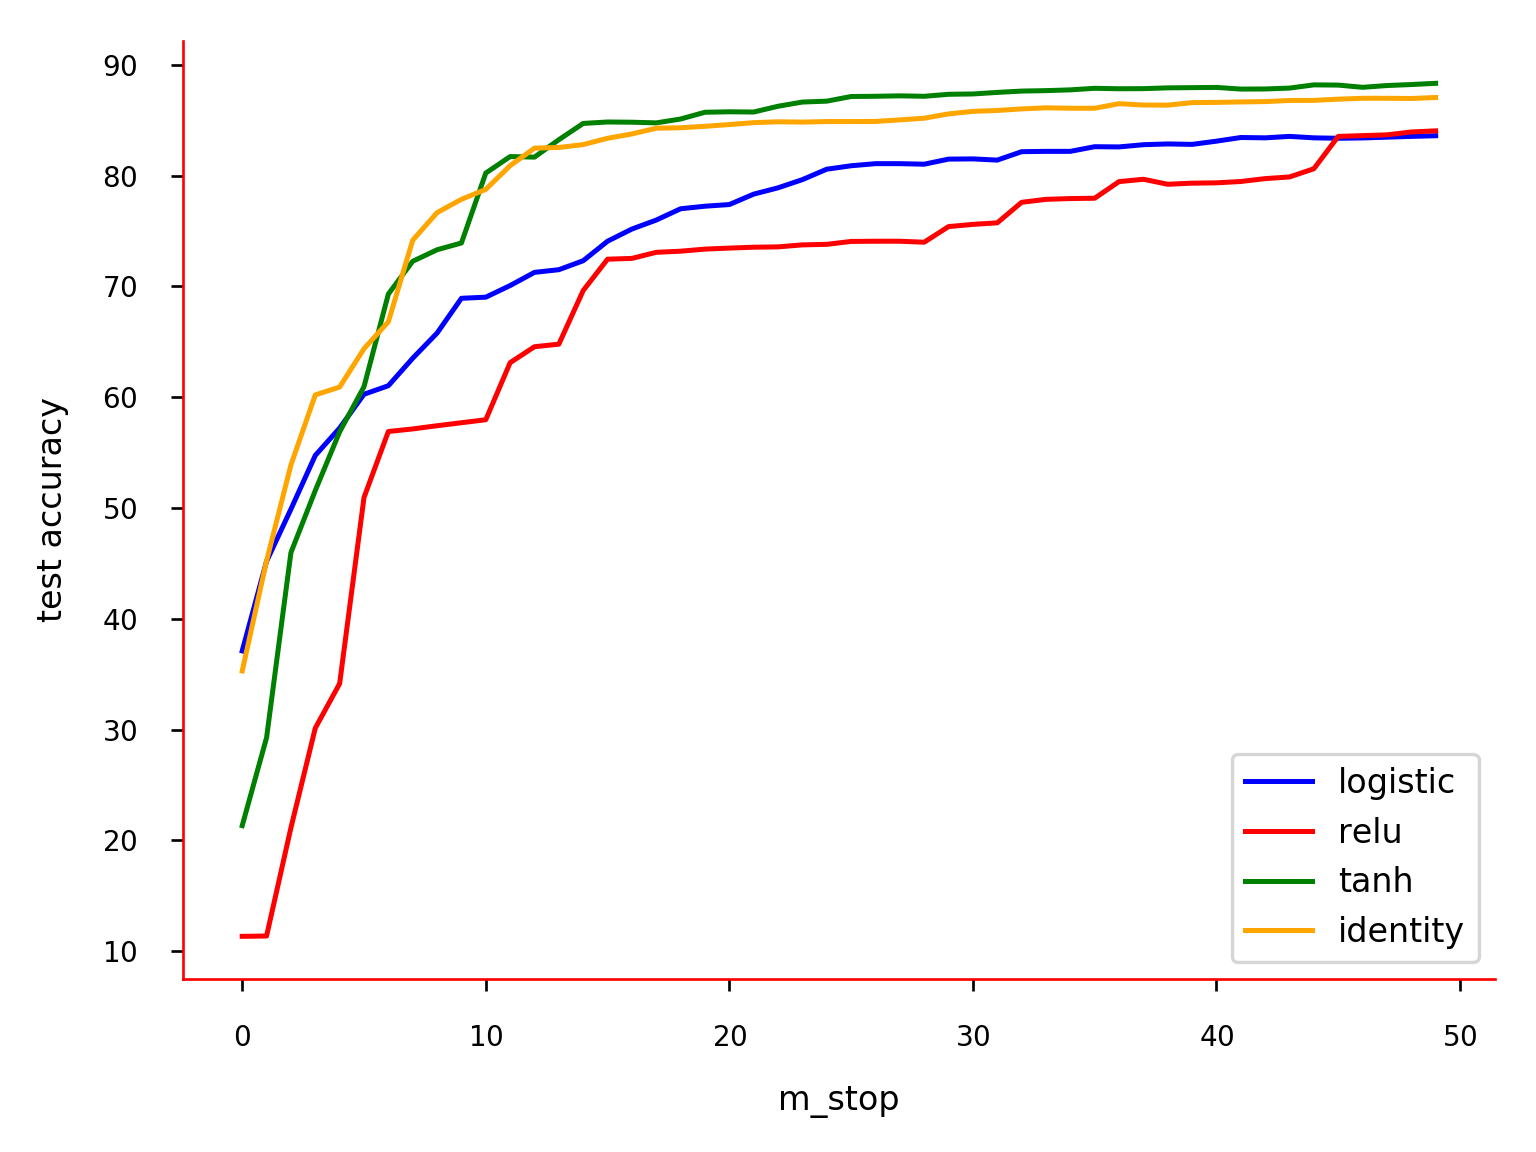
\includegraphics[width=0.9\textwidth]{includes/boosting-comparison-plot.png}
			\caption{Test accuracy versus the number of trained nodes in an incrementally trained network}
			\label{fig:boosting-comp-plot}
		\end{figure}

		Since in this case, the hypothesis space is closed under scalar multiplication (as the scalar will get multiplied only to the weights incoming on the output layer, which does not disturb the hypothesis class), we can set the objective as given in equation \ref{eq:weak-obj-closed}. Since the objective is given for the data distribution which is not known, we replace the objective by an empirical objective, where the optimization is only over the data points belonging to the sample set $\cS$. Since our objective is a linear regressor, we choose the norm to be a l$_2$ norm. Therefore, our final objective becomes a simple least squares objective, given as
		\begin{align*}
			h_m \qdeq \argmin{h \in \cH} \sum_{(\vx, y) \in \cS} \norm{g(\vx, y) - h(\vx, y)}_2^2
		\end{align*}

		In Figure \ref{fig:boosting-comp-plot}, we have shown the performance of the said boosted system, or equivalently, an incrementally trained neural network. It is clear that each individual weak learner we have chosen is embarrassingly weak, yet the performance of the trained network is decent on the dataset. However the performance does not compare well with that of a neural network trained using the backpropogation scheme, which gives over 95\% test accuracy. Therefore, even for a simple example, we can conclude that incremental training gives poorer results when compared to the collective training of a network.

	\end{psubsection}

	\begin{psubsection}{Incremental Training as a Pre-Training Step}

		Training of a neural network, or any model can be broken into two parts, pre-training and fine-tuning. For most tasks, the pre-training is skipped, and the weights are initialized using random values, therefore only the notion of fine-tuning remains.

		Working on the hypothesis that the boosted model, or the incrementally trained neural network can be a good initialization (or pre-training), we performed experiments on the same classification task, with the incrementally trained neural network as a pre-training step for the network, and then applying the standard backpropogation over this pre-trained network for the purpose of fine-tuning.

		The final test accuracies for each case has been reported in Table \ref{tab:accuracies-mnist}. It can be seen that there are marginal improvements on the test accuracies in the case of networks which have been incrementally pre-trained. This suggests that the pre-training, although does not change the performance by a lot, can improve performance marginally, which might be helpful in cases where the predictions are extremely sensitive, for example Cancer detection.

		\begin{table}[h!]
			\centering
			\begin{tabular}{|L{3cm}|C{2.5cm}|C{2.5cm}|c|}
				\hline
				\bt{Activations}	&	\bt{Incremental}		&	\bt{Collective}		&\bt{Pre-trained + Fine-tuned}	\\
				\hline
				sigmoid				&	85.000000				&	97.110000				&	97.460000					\\
				relu				&	84.900000				&	96.980000				&	97.310000					\\
				tanh				&	87.840000				&	96.450000				&	96.950000					\\
				identity			&	85.640000				&	91.710000				&	91.820000					\\
				\hline
			\end{tabular}
			\caption{Test Accuracies for Differently Trained Neural Networks}
			\label{tab:accuracies-mnist}
		\end{table}

		We explicitly perform experiments on the class imbalance case, with the Iris dataset where the imbalance is manually induced. The results for the same are shown in Table \ref{tab:accuracies-iris}. It can be clearly seen that the accuracies obtained in the case of collectively trained neural network are embarrassingly low. We also ran the training of the network multiple times with an extremely low tolerance to ensure the convergence, however the network always seemed to converge with a similar final accuracy. This could be explained by the convergence of the network to a local optima, since the objective is highly non-convex. Whereas, the pre-trained neural network seems to avoid this local optima, and converge to a better optima.

		\begin{table}[h!]
			\centering
			\begin{tabular}{|L{3cm}|C{2.5cm}|C{2.5cm}|c|}
				\hline
				\bt{Activations}	&	\bt{Incremental}		&	\bt{Collective}		&\bt{Pre-trained + Fine-tuned}	\\
				\hline
				sigmoid				&	78.181818				&	76.363636			&	94.545455					\\
				relu				&	97.272727				&	45.454545			&	97.272727					\\
				tanh				&	81.818182				&	48.181818			&	97.272727					\\
				identity			&	98.181818				&	92.727273			&	97.272727					\\
				\hline
			\end{tabular}
			\caption{Test Accuracies for Differently Trained Neural Networks}
			\label{tab:accuracies-iris}
		\end{table}

		We confirmed this hypothesis by reducing the number of nodes in the collectively trained neural network, and observed a boost in accuracy. This strongly suggests that the added non-convexity due to larger number of nodes was preventing the network to converge to the global optima. Whereas, the pre-trained network did not have this problem even with a large number of nodes, since the network is already close to a decent optima, local or global.

	\end{psubsection}

	\begin{psubsection}{Mini-Batch Training --- Stronger Weak Learners}

		One problem with the pre-training that is easily observable is that the training takes a lot of time, and in case of marginal performance boosts, one might simply prefer the collective training model for the sake of saving time. We further extend the training to a mini-batch setting in order to decrease the total time of training, while maintaining the lower non-convexity for each weak learner.

		The idea of a mini-batch is to allow multiple nodes in one weak learner, and reduce the total number of stops (or boosted weak learners) so as to keep the total number of nodes. Since the strength of each weak learner is greatly improved, it will converge to a better accuracy. Also, since the collective training of a neural network takes lesser time, the total time is expected to be lesser than the time spend boosting single node single hidden layer networks.

		However, increasing the number of nodes in a single weak learner increases the non-convexity of each learner, however, if we limit the number of nodes in a weak learner to a small value (say $< 5$), then we can almost always ensure that each weak learner will converge to its global optima. This allows us to decrease the total pre-training time, while ensuring similar convergence guarantees.

		This remains a hypothesis, and we could not this due to shortage of time, but we leave this approach for future exploration.

	\end{psubsection}

\end{psection}

\begin{psection}{Conclusion}

	In this project report, we have discussed the Gradient Boosting algorithm for convex objectives, applied it to sequentially train the nodes of a single hidden layer neural network and derived empirical results on different weak learners as node activations. The results are summarized in Table \ref{tab:accuracies}.

	There are a few observations worth noting. The improvement that was anticipated as a result of the warm start provided by incremental training of nodes is appreciable, and is attributed to provable convergence guarantees of a boosted model which allows the neural network to converge to a better optima.

	Further, the pretraing method may induce structure in the individual activations of the nodes thereafter trained. This mode of training is vaguely similar to the greedy layer-wise approach in Deep Boltzmann Machines, though in this case the greedy approach is applied to single layer among the nodes. We also propose the mini-batch training, which could help in reducing the pre-training time while maintaining the good convergence properties of the sytem.

	We also notice from Figure \ref{fig:boosting-comp-plot} that as the number of weak learners increase, the accuracy obtained slowly saturates to a suboptimal level compared to vanilla backpropagation. We may apply early stopping in this case to infer the number of nodes ideal to a layer in the network, which can be then fine tuned to yield better results.

	Further work in this regard, in the direction of multi-layer pretraining using gradient boosting, may lead to efficient inference of model complexity and better warm starts. The problem that may arise in such a case is that objectives are no longer convex for the boosting procedure, giving us no such convergence guarantees for this methods. This remains a promising avenue for exploration, one that may benefit from advances in the developing theory of nonconvex optimization techniques.

\end{psection}

\bibliographystyle{plainnat}
\bibliography{report}

\end{document}
